\documentclass{article}
\usepackage[utf8]{inputenc}
\usepackage[english]{babel}
\usepackage[utf8]{inputenc}
\usepackage{fancyhdr}
\usepackage{graphicx}

\begin{folding}
\title{SLM Circuit Simulator Log}
\author{Sam Taylor, Maximus Wickham , Leonardo Garofalo}
\date{June 2020}

\pagestyle{fancy}
\fancyhf{}
\rhead{SLM Soloutions}
\lhead{SLM Circuit Sim}
\rfoot{Page \thepage}
\end{folding}
\graphicspath{ {./images/} }
\begin{document}

\maketitle
\tableofcontents
\newpage

\section{Engineering Design Process}
\flushleft

\subsection{Outline of technical problem to be solved:}
\flushleft

\smallbreak
Write a software package that performs a transient simulation of a circuit, like LTspice. The main elements of such a system are described below:
\newline
\smallbreak
1. Parse the netlist file using reduced SPICE format.
\newline
2. Set up the simulation (Transient Analysis , DC Bias Point Analysis)
\newline
3. Construct and solve the conductance matrix
\newline
4. Process voltage sources
\newline
5. Write the output
\newline
6. Add support for non-linear components (advanced)
\newline
\mediumbreak 

Key Evaluation points:
\newline
1. Accuracy: compare the outputs to pen and paper solutions. 
\newline
2. Efficiency: find how long the simulation takes and, by estimating the power consumption of your computer.

\subsection{Software Requirements Specification:}
\flushleft
\textbf{Outline:} A circuit Simulation that produces transient analysis for circuits containing energy storage devices , diodes and transistors . With reasonable accuracy and speed.

\bigbreak

\textbf{Functional Requirements}

\newline

1. Give Node Voltages of a complete circuit within 1 percent of Spice
\newline
2. Evaluate Current flowing through each component within 1 percent of Spice
\newline
3. Perform analysis for passive, energy storage devices , diodes and transistors.
\newline
4. Take input from a reduced spice netlist file.
\newline
5. Output analysis to an output file.
\newline
6. The software must be capable of dealing with both linear and non-linear devices

\bigbreak

\textbf{Non-Functional Requirements}
\newline
1.The software must be capable of analyse different kinds of circuits
\newline
2. The software must be able to perform the analysis in a fast and efficient way
\newline
3. The software must be capable of performing the analysis consuming the least amount of power possible

\newpage

\subsection{High Level Design}
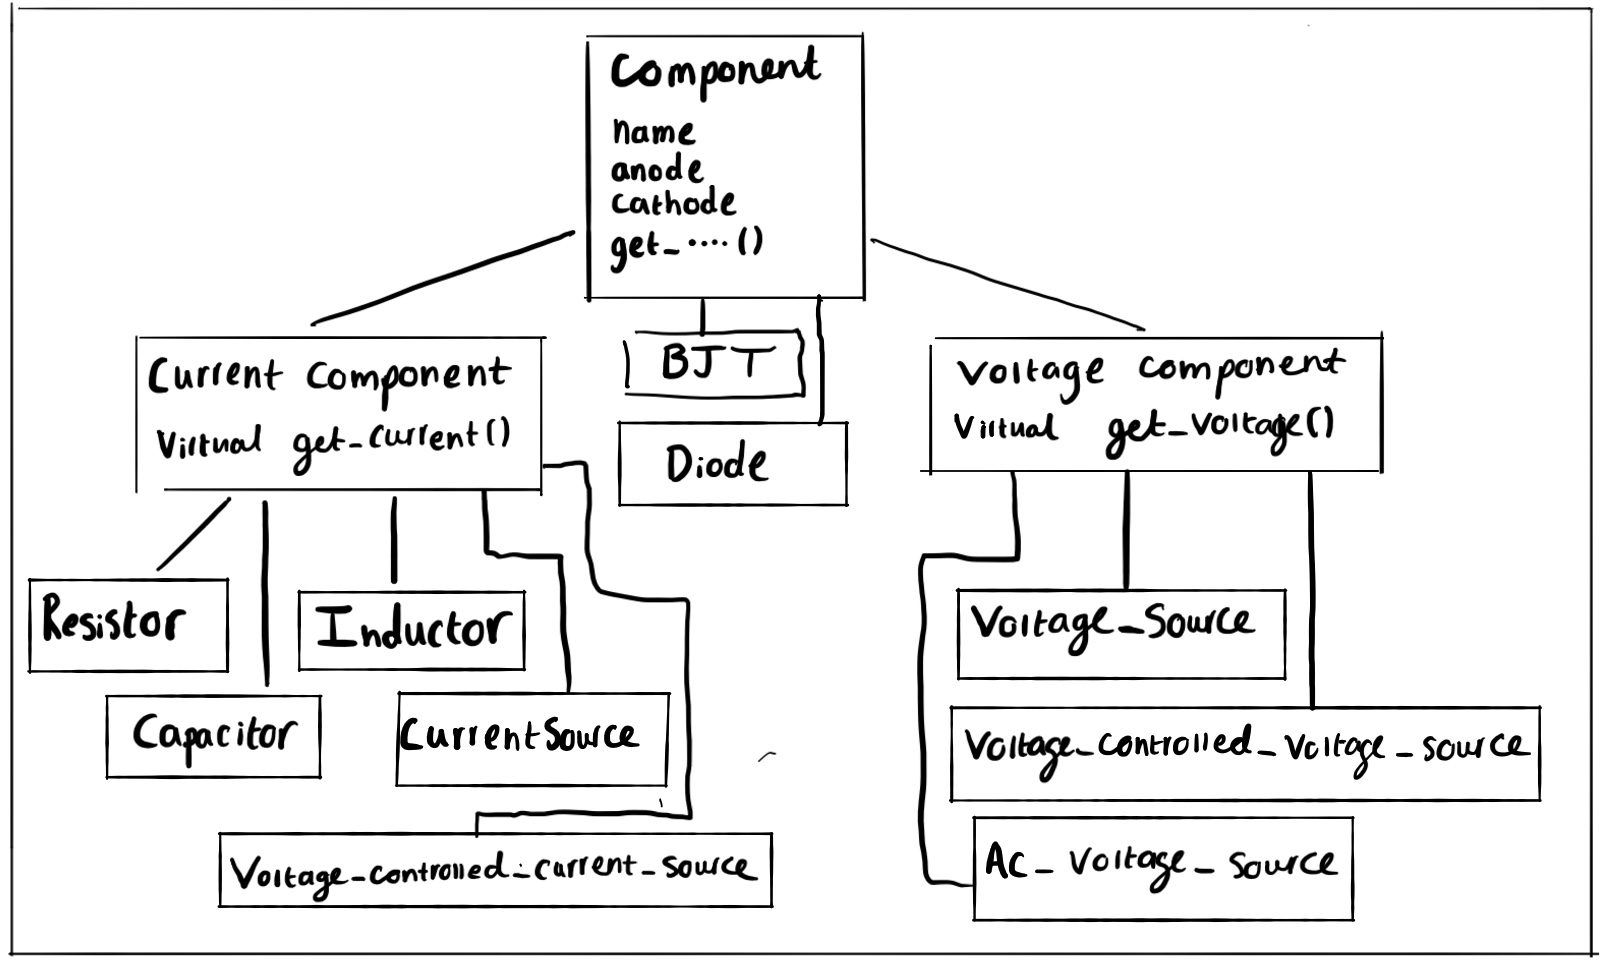
\includegraphics[width=15cm]{images/AlgoDesStr2.jpg}
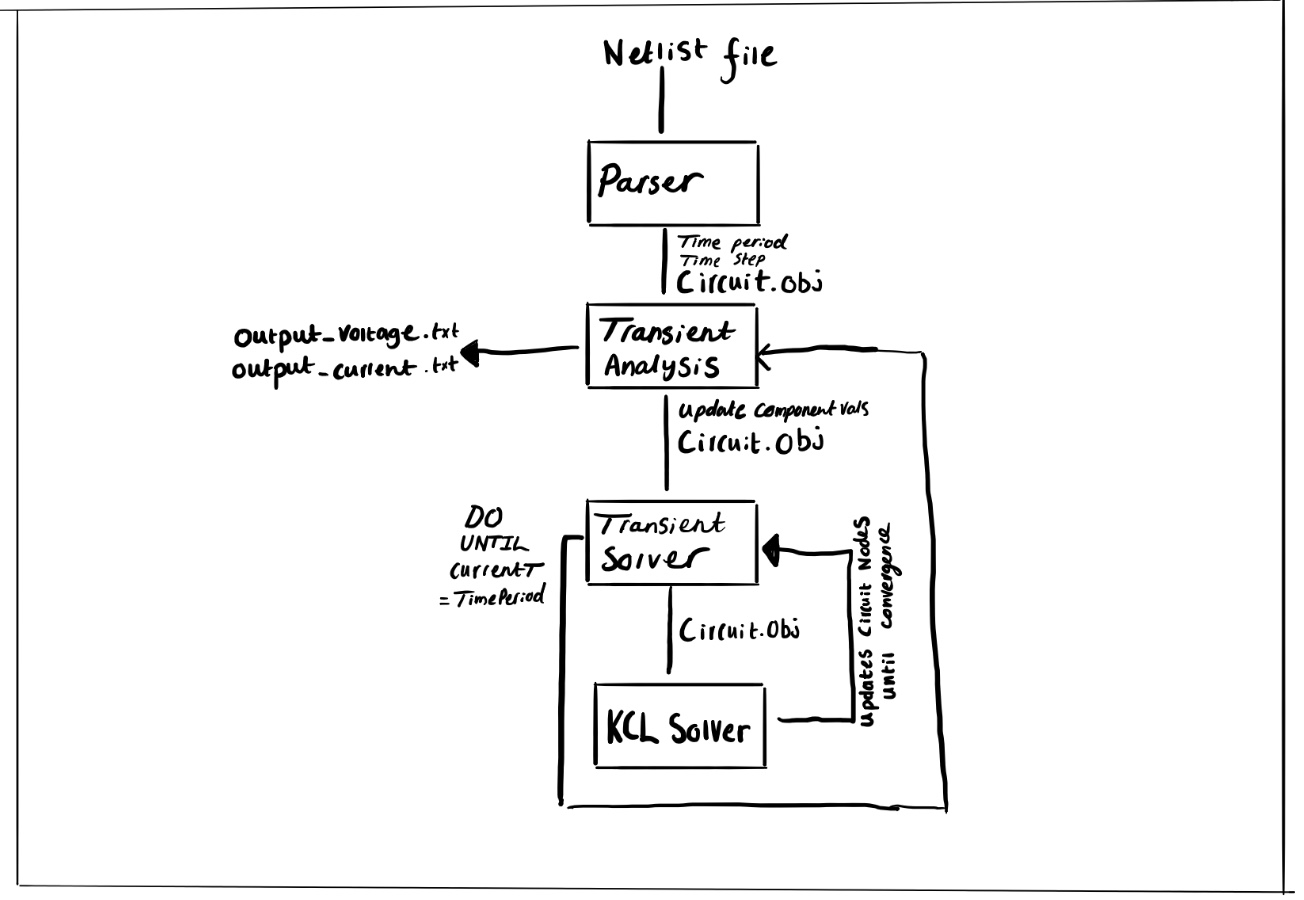
\includegraphics[width=15cm]{images/Comphpp.jpg}


\section{High Level Design}

\newpage

\section{Component Models}

\newpage

\section{Analysis Algorithms}

\newpage

\section{Application Features}

\newpage

\end{document}
